% Hermes-3 solver optimisation: a short deck for an external audience.
% Built with: xelatex design-summary-slides.tex
% The figure comes from the project's own report generator.

\documentclass[aspectratio=169,11pt]{beamer}

\usetheme{default}
\usecolortheme{seahorse}
\setbeamertemplate{navigation symbols}{}
\setbeamertemplate{footline}[frame number]
\setbeamerfont{frametitle}{size=\large}
\setbeamercolor{frametitle}{fg=black}
\setbeamertemplate{itemize items}[circle]
\setlength{\parskip}{4pt}

\usepackage{fontspec}
\usepackage{graphicx}
\usepackage{booktabs}

\title{Optimising the Hermes-3 solver}
\subtitle{Searching PETSc settings for tokamak edge simulations}
\date{20 September 2026}

\begin{document}

\begin{frame}
  \titlepage
\end{frame}

\begin{frame}{The problem}
  Hermes-3 simulates the plasma edge of a tokamak: how a reactor's exhaust
  cools before it reaches the wall.

  \begin{itemize}
    \item Stiff equations, so the solve is implicit. PETSc SNES, every timestep.
    \item Nearly all the cost sits inside that solver.
  \end{itemize}

  \vspace{0.4em}
  Measured on our own cases:

  \begin{itemize}
    \item 100\,ms of plasma took \textbf{16.6 hours} on ten cores.
    \item That is about 145\,ms of plasma per day of wall clock.
    \item Steady state: days to weeks. A study needs tens of cases.
  \end{itemize}

  \vspace{0.4em}
  The solver's speed decides which physics questions are askable at all.
\end{frame}

\begin{frame}{Fifty settings, chosen by hand}
  \begin{itemize}
    \item Tolerances, Jacobian reuse, linear solver, preconditioner, timestep control.
    \item Picked from intuition, by a handful of people, over years.
    \item Nobody has searched the space.
  \end{itemize}

  \vspace{0.6em}
  Our records: four configurations across 48 runs.
  Throughput spans a \textbf{factor of three} on one test case.

  \vspace{0.6em}
  A two-fold speed-up turns a week of waiting into three days --- on every
  study that follows, for every user of the code.
\end{frame}

\begin{frame}{Where the time actually goes}
  \begin{center}
    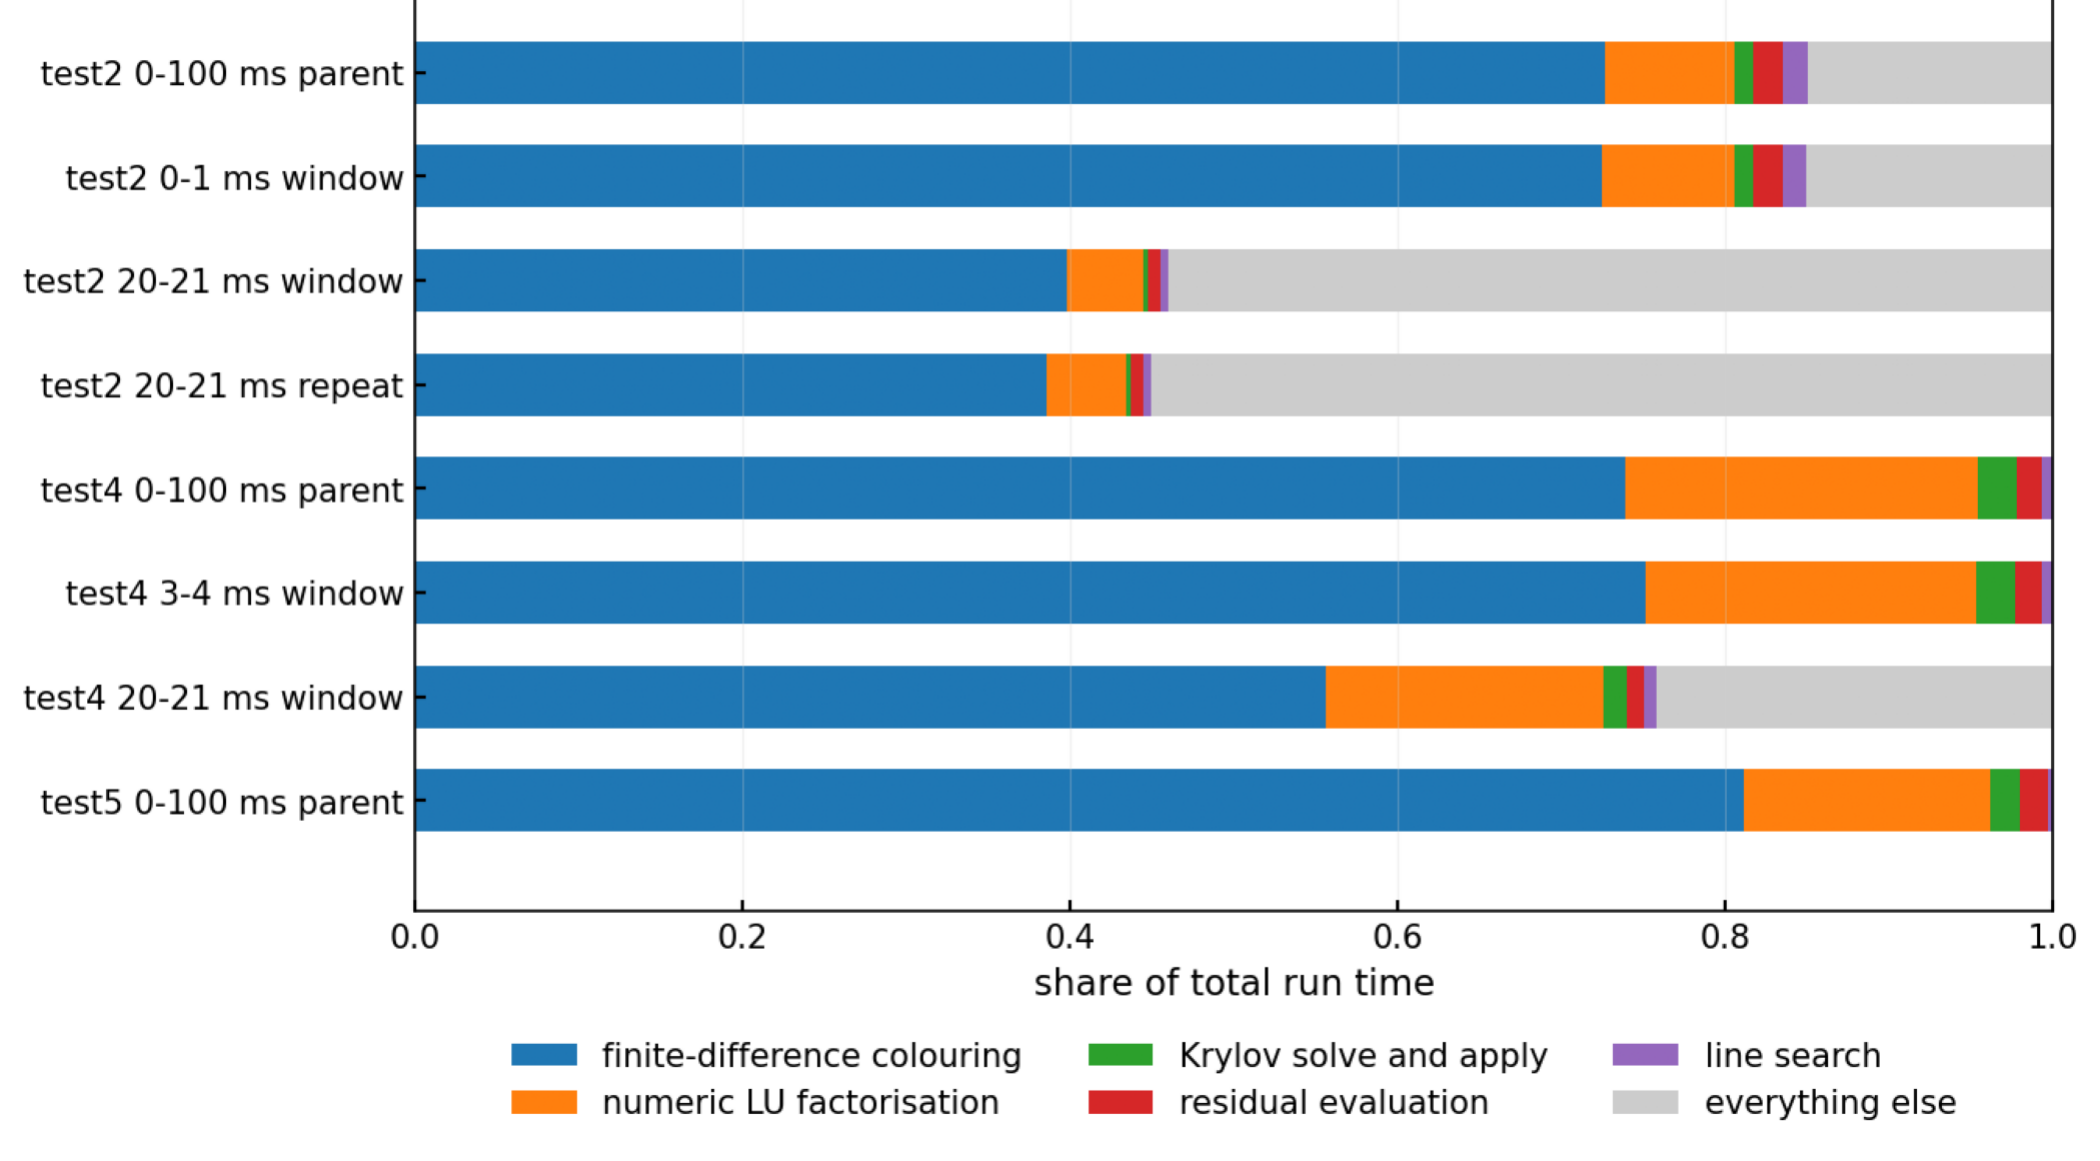
\includegraphics[width=0.70\textwidth]{design-summary-cost-breakdown.png}
  \end{center}

  \vspace{-0.2em}
  \begin{center}
    Jacobian colouring \textbf{73--81\%} \quad$\cdot$\quad LU 5--22\%
    \quad$\cdot$\quad Krylov under 3\%
  \end{center}

  {\small The exact LU converges in one iteration, so the Krylov layer is
  nearly all overhead.}
\end{frame}

\begin{frame}{The search space}
  Six groups, about fifty knobs:

  \begin{columns}[T]
    \begin{column}{0.48\textwidth}
      \begin{itemize}
        \item Nonlinear solve
        \item Jacobian
        \item Variable scaling
      \end{itemize}
    \end{column}
    \begin{column}{0.48\textwidth}
      \begin{itemize}
        \item Linear solve
        \item Preconditioner
        \item Timestep control
      \end{itemize}
    \end{column}
  \end{columns}

  \vspace{0.6em}
  Mixed types: switches, choices, integers, continuous over decades.

  \vspace{0.4em}
  \textbf{And conditional.} The factorisation package means nothing unless the
  preconditioner is a direct solve. The PID gains mean nothing unless the
  controller is the PID one.

  \vspace{0.4em}
  A sampler that ignores that structure spends its budget on settings that are
  not in force.
\end{frame}

\begin{frame}{Defaults are not choices}
  We captured what PETSc \emph{actually built}, not what the input file says.

  \vspace{0.6em}
  \begin{center}
    \large
    GMRES restart $= 30$ \qquad against \qquad iteration cap $= 260$
  \end{center}

  \vspace{0.4em}
  So one solve can restart nearly nine times, discarding its convergence
  history each time.

  \vspace{0.6em}
  Nobody chose 30. It is PETSc's default and the input file never mentions it.

  \vspace{0.6em}
  Building the space description from the running code, rather than from the
  input file, surfaces these immediately.
\end{frame}

\begin{frame}{Making an evaluation cheap}
  We do not evaluate a configuration on a whole simulation. We evaluate it on a
  slice.

  \begin{itemize}
    \item One \textbf{parent run} per test case: 0--100\,ms, fixed build, saves state every ms.
    \item Cut \textbf{seeds} from it: restart files at chosen times.
    \item A \textbf{window} restarts from a seed and runs to a later time.
  \end{itemize}

  \vspace{0.4em}
  \begin{center}
    \begin{tabular}{llr}
      \toprule
      Rung & Windows & Noise bound \\
      \midrule
      0 & three, 0.2--0.5\,ms & 15\% \\
      1 & the same three, $4\times$ longer & 10\% \\
      2 & the full 100\,ms run & 5\% \\
      \bottomrule
    \end{tabular}
  \end{center}

  \vspace{0.4em}
  Positions probe the flat-start transient, the approach to steady state, and
  near-steady state.
\end{frame}

\begin{frame}{Why we do not trust windows by rank}
  A configuration can be slow early and fast late. No single window predicts the
  full run.

  \vspace{0.6em}
  So instead of rank correlation:

  \begin{itemize}
    \item Each window measures a \emph{speed} at its position in the run.
    \item Full-run cost = sum of each stretch at its local speed.
    \item A real full run checks the estimate periodically.
    \item Promote generously --- cheap rungs cannot see a slow divergence.
  \end{itemize}

  \vspace{0.8em}
  \textbf{We have not found this published.} Restart windows of one simulation
  as fidelity levels appears to be novel. We would like the argument attacked.
\end{frame}

\begin{frame}{Fast for the wrong reason}
  A configuration can be fast because it takes sloppy steps and converges to the
  wrong plasma. Timing never reveals that.

  \vspace{0.6em}
  Correctness is a \textbf{pass/fail flag beside the cost}, never a term inside
  the objective.

  \begin{itemize}
    \item Window check, every rung: sanity band on four physical quantities.
          Failing disqualifies. Passing proves little.
    \item Endpoint check, full runs only: same steady state as the reference?
          This is the verdict that counts.
  \end{itemize}

  \vspace{0.6em}
  Outcomes are a fixed, script-decidable taxonomy. A crash never scores as slow.
  A timeout is evidence, not a missing result.
\end{frame}

\begin{frame}{The record}
  One row per run, about fifty columns, append-only, in git. Per-run evidence
  sits beside it, outside git.

  \vspace{0.6em}
  Three rules:

  \begin{itemize}
    \item \textbf{The index defines what exists.} No enumerating directories.
    \item \textbf{Nothing is typed twice.} Intent before the run, measurement
          after. An undeclared difference gets flagged.
    \item \textbf{Nobody reads fifty columns.} Queries return about ten,
          filtered and ranked --- counting across a wide table is exactly where
          both people and models fail.
  \end{itemize}
\end{frame}

\begin{frame}{Two layers, one narrow interface}
  \begin{columns}[T]
    \begin{column}{0.48\textwidth}
      \textbf{Runner}
      \begin{itemize}
        \item Plain command-line program.
        \item No judgement in it.
        \item Prepares, launches, watches, extracts, repeats.
        \item Runs unattended.
      \end{itemize}
    \end{column}
    \begin{column}{0.48\textwidth}
      \textbf{Optimiser}
      \begin{itemize}
        \item Decides what to try next.
        \item Model, sampler, or a person with a list.
        \item The runner cannot tell which.
      \end{itemize}
    \end{column}
  \end{columns}

  \vspace{0.8em}
  \begin{center}
    Interface: \emph{suggest trials} $\rightarrow$ \emph{report results}
  \end{center}

  \vspace{0.4em}
  Swapping the optimiser changes nothing else.
\end{frame}

\begin{frame}{What the evidence says about model optimisers}
  Reviewed September 2026. Genuinely mixed:

  \begin{itemize}
    \item Value is in \emph{proposing} when data are sparse, not in predicting.
          As a predictor a model loses to standard surrogates.
    \item Budget-matched study, June 2026: the advantage was mostly a sensible
          starting configuration. Seeded random search tied at five evaluations,
          won by twelve.
    \item Eleven-simulator benchmark, March 2026: 66--81\% success, but
          1.5--2.7$\times$ the compute of plain scanning.
    \item They stagnate rather than converge. A fallback is not optional.
  \end{itemize}

  \vspace{0.5em}
  Our reading: best as a \textbf{cold-start proposer} and a \textbf{reader of
  failures}, not as the search algorithm.

  \vspace{0.3em}
  So: run controls, show at most $\sim$30 past trials, validate output against a
  schema before launching, fall back to the sampler on drift.
\end{frame}

\begin{frame}{Open questions}
  \begin{enumerate}
    \item \textbf{Is the window ladder sound?} Unpublished, and the obvious
          objection is that a short window does not predict a long run. We answer
          with speed-summation rather than rank correlation. Attack it.
    \item \textbf{How to map a mixed, conditional space?} Fifty knobs, four
          types, dependencies switching whole groups on and off. No principled
          answer yet.
    \item \textbf{Right objective for steady state?} Work to reach a residual
          level, not to reach a fixed simulated time --- especially for
          pseudo-transient methods. Unreconciled with the window ladder.
    \item \textbf{Are the cheap rungs too cheap?} Shortest windows cost 9 and
          20 seconds. Almost certainly below the noise floor.
  \end{enumerate}
\end{frame}

\begin{frame}{Status}
  \textbf{Works today}
  \begin{itemize}
    \item Measurement layer: log and dump $\rightarrow$ row and bundle, verified against a live run.
    \item Record: nine runs on a fixed build, documented schema, re-derivation check.
    \item Parent runs for three test cases; seed library for two.
    \item Window generator.
  \end{itemize}

  \vspace{0.5em}
  \textbf{Designed, not built}
  \begin{itemize}
    \item The runner loop, the campaign config, and any optimiser at all.
  \end{itemize}

  \vspace{0.5em}
  \textbf{Caveat we are honest about}

  The variable rescaling floors small elements at the solver's relative
  tolerance. We measured it: the floor is reached in 14 of 16 runs. Until we
  know what share of the residual norm those elements carry, residual-based
  objectives are not safe to tune against.
\end{frame}

\end{document}
